\documentclass{article}

\usepackage{pdfpages}
\usepackage[utf8]{inputenc}
\usepackage{eurosym}
%\usepackage{fancyhdr}
%\pagestyle{fancy}

%
%Die eingegangenen Projektskizzen werden nach folgenden Kriterien bewertet:
%– Zielabdeckung: Das Vorhaben ist auf die Vermittlungsziele des Wissenschaftsjahres 2019 zugeschnitten (Berück-
%sichtigung der Handlungsfelder, Zielgruppen, Forschungsinhalte).
%– Fachliche Kompetenz: Der Antragsteller ist qualifiziert, das Vorhaben durchzuführen und verfügt über nachgewie-
%sene Expertise über das Themenfeld und/oder die Vermittlung des Themenfelds.
%– Schlüssigkeit und Konsistenz des Konzepts: Idee, Ziele, Budgetschätzung.
%– Kommunikative Ausrichtung und Wirksamkeit: Das Vorhaben wird von geeigneten Kommunikationsmaßnahmen be-
%gleitet, es ist öffentlichkeitswirksam und generiert voraussichtlich eine mediale Berichterstattung. Das Vorhaben wird
%kommunikativ in das Wissenschaftsjahr 2018 eingebunden und als Teil dessen wahrgenommen.
%– Innovation: Das Vorhaben ist innovativ und leistet einen Beitrag zur Weiterentwicklung der Wissenschaftskommuni-
%kation in Deutschland.
%– Überregionalität und Nachhaltigkeit: Das Vorhaben strahlt überregional aus und/oder kann übertragen bzw. nachgenutzt werden


\begin{document}


\begin{center}
%\vspace{-13cm}
{ \centering 
\includegraphics[width=10cm]{hsf.png} }

\vspace{-0.8cm}
\begin{figure*}[h!]
\centering
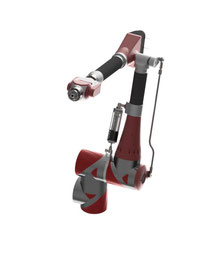
\includegraphics[width=0.6\textwidth]{arm.png}
\end{figure*}
\vspace{-1.8cm}

{\Huge\bf
PROJEKTSKIZZE: Lernen in Handarbeit
}
\\[2em]
\Large
{\bf Antragsteller:} Prof. Dr. Alexander Gepperth (HDR)\\
{\bf Adresse: } Fachbereich Angewandte Informatik der HAW Fulda\\
Leipzigerstr. 123, 36037 Fulda\\
{\bf Email: } alexander.gepperth@cs.hs-fulda.de\\
{\bf Telefon: } 0661 9640 3485\\
\vspace{0.5cm}

{\bf Projektdauer:} 9 Monate\\
\vspace{0.5cm}

{\bf Gesamtkosten:} 150.000\euro\\
\vspace{0.5cm}

{\bf Zuwendungsbedarf:} 150.000\euro\\
\vspace{0.5cm}

%{\bf Konsortium:} Assisted Living, Hilfe für Schwerbehinderte, Service-Robotik, 3D-Simulation
\end{center}
%\end{titlepage}
\newpage

\renewcommand{\thesection}{2}
\section{Antragsteller und assoziierte Partner}
Projektleiter des Projektes ist Herr Prof. Dr. Alexander Gepperth. Prof. Gepperth hat Kompetenzen/Erfahrung/Projekte etc...

\renewcommand{\thesection}{3}
\section{Ausgangsfrage und Ziele des geplanten Vorhabens}

\begin{itemize}
	\item Ziel: Demonstratorsystems zur Visualisierung der Funktionsweise des überwachten Lernens mittels NN
	\item Aufbau eines Handgestenerfassungs + Croppingsystems
	\item Einspeisung + Visualisierung der erfassten Daten für die Benutzer
	\item Visualisierung der Klassifikationsgüte (schlecht - mittel - gut)
	\item Darstellung der Dateneinspeisung, des Trainings, der Veränderung des Netzes + der Verbesserung der Klassifikationsgüte: Lernen durch Beispiele
	\item Deep Dreaming
	\item Handposen vs. Handgesten
	\item Forschungsaspekt: Inkrementelles Lernen

\end{itemize}


\subsection{Kurzzusammenfassung}
Das Projekt hat zum Ziel, ein interaktives Demonstrationssystem zur Veranschaulichung der Arbeitsweise maschinellen Lernens zu erstellen. 
Gegenstand des Lernens sind Handposen, die dem System interaktiv durch direkte Demonstration vermittelt werden, bzw. welche das System nach
erfolgter Demonstration klassifiziert, wobei nach jeder Klassifikation der interne Zustand des Lernverfahrens visualisiert wird, welcher zu einer Entscheidung geführt hat. 
Die hauptsächlichen Erkenntnisse zum maschinellen Lernen, welche vermittelt werden sollen, lauten wie folgt: zunächst soll kalrgemacht werden, dass maschinelles Lernen nicht unfehlbar ist, sondern
Fehler machen kann, was vor allem dann geschieht, wenn Anzahl und Qualität der Daten unzureichend ist. Weiterhin soll durch eine anschauliche Visualisierung des internen Zustands der LErnverfahrens erreicht werden, dass die grundsätzliche Arbeitsweise solcher Lernverfahren keine "schwarze Magie" darstellt, sondern auf anschaulicher Ebene  verstanden werden kann. 
%Zu guter Letzt soll der Demonstrator dazu dienen, fundamentale Konzepte des maschinellen Lernens, wie z.B. Generalisierung oder Überanpassung, auf anschauliche Art zu verdeutlichen. 
Zu guter Letzt soll mit den im Laufe der Demonstration trainierten Handposen eine Applikation oder ein Spiel gesteuert werden, um zu verdeutlichen dass maschinelles Lernen auch großes Potential
für Unterhaltung und Amüsement in sich trägt. 
%
\subsection{Grundsätzliche Zielsetzung}
%
Maschinelles Lernen wird in er populären Wahrnehmung vielmals als mathematisch komplex und für Laien unverständlich wahrgenommen. Da maschinelle Lernverfahren in zunehmender Weise über Aspekte unseres täglichen Lebens entscheiden (z.B. bei der Kreditvergabe), führt diese Intransparenz nach unserer Auffassung dazu, das Misstrauen gegenüber maschinellen Lernverfahren zu erhöhen. Dem kann entgegengewirkt werden, indem gerade jungen MEnschen vermittelt wird, dass
die grundsätzliche Funktionsweise solcher Verfahren einfach nachzuvollziehen ist, sowie dass die Fähigkeiten von Lernverfahren fast ausschließlich von den Daten abhängen, mit denen sie trainiert werden. Das Ziel soll sein, dass maschinelle Lernverfahren als das gesehen werden was sie sind: als Werkzeuge, deren Funktionsweise man verstehen kann, statt als intransparente Entscheider. 
Das wird erreicht, indem Benutzergruppen in die Lage versetzt werden, ihr "eigenes" Lernverfahren durch direkte Demonstration zu trainieren, wobei live visualisiert wird, {\it warum} ein Verfahren zu einer bestimmten Entscheidung kommt.
%
\renewcommand{\thesection}{4}
\section{Ausführliche Vorhabensbeschreibung}
\subsection{Einsatzszenario}
An der HAW Fulda existieren multiple Formate des Austauschs mit lokalen Schulen und der interessierten Öffentlichkeit: MINTMachClub\footnote{mint},Kinder-Universität\footnote{ku}, MINT-Labortage\footnote{mlt} sowie
reguläre Besuche von Schulklassen, oft aus der gymnasialen Oberstufe zur Hinführung auf ein mögliches Studium. Generell ist maschinelles Lernen für diese Zielgruppen sehr interessant und dessen Sinnhaftigkeit leicht vermittelbar, weswegen sich Präsentationen bzw- Demonstrationen für diese Zielgruppen oft überschneiden und wiederholen, was ein standardisiertes Format sinnvoll macht. 
Weiterhin ist allen Zielgruppen gemein, dass sie eher durch interaktive Lerhformate angesprochen und begeistert werden können, speziell in den niedrigeren Klassen. Hierbei macht es sicherlich Sinn, die Demonstration flexibel gestalten zu können:
rein interaktiv und relativ kurz für Schüler*innen ohne Informatik-Erfahrung, oder per API programmierbar für Oberstufenklassen im Rah,en eines Vormittagsprojekts. 
%
\subsection {Ablauf einer Demonstration}
Als Zielgruppe einer Demonstration wird eine Gruppe von 10 Personen oder mehr angenommen. Der erste Abschnitt besteht aus der gemeinsamen Definition der 
zu benutzenden Handposen. In der zweiten Phase demonstrieren bis zu 10 Personen gleichzeitig, auf Aufforderung des Demonstrators, einzelne Handposen, welche von Demonstrator registriert 
und zum Training der maschinellen Lernverfahrens genutzt werden. In der folgenden dritten Phase demonstrieren einzelne PErsonen Handposen, für welche der Demonstrator seine Klassifikationen ausgibt und
ausführlich visualisiert (Einzelkonfidenzen, Gesamtkonfidenz), wie diese Entscheidung zustande gekommen ist. Phasen 2 und 3 können beliebig oft wiederholt und der LErnfortschritt verglichen werden. Durch die Wiederherstellung vergangener Zustände und systematische Manipulation der gezeigten Handposen können verschiedene typische Effekte für fortgeschrittene Zielgruppen gezielt demonstriert werden, vor allem Overfitting und Generalisierung. 
%
Als letzte Demonstrationsphase sollen die Teilnehmer die dem System antrainierten Handposen nutzen, um eine Anwendung zu kontrollieren, wobei sich
die Steuerung eines Spiels bzw die Steuerung eines autonomen Roboters anbieten. Auch eine zur Verfügung Stellung der erkannten Handposen per ReST API ist denkbar, 
wobei dann die Reaktion eines Computersystems auf eine bestimmte Handpose von fortgeschrittenen Teilnehmern im Rahmen einer Projetkarbeitsphase selbst programmiert werden kann.
%
lernen der einschränkungen: linek hand trainieren, rechte testen --> problem!
\subsection{Technische Bausteine der Demonstration}
Für die 
{\bf 3D-Datenanalyse}
{\bf Handposenerkennung und Klassifikation}
{\bf Visualisierung}
message: ist nur ein verfahren, keine Magie
%
\renewcommand{\thesection}{5}
\section{Darstellung des Eigeninteresses/Eigenanteils}
%
Die HAW Fulda hat tiefgehende Kompetenzen im Bereich des Maschinellen Lernens und modernen Interaktionstechniken. Im Bereich der modernen Interaktionstechniken (insb. Freihandgesten) wurde in bilateralen Forschungsvorhaben ein Demonstrator zur Erkennung von Handgesten mittels 3D-Sensorik entwickelt. Mit Hilfe dieses Demonstrators konnten zahlreiche Erkenntnisse im Bereich des überwachten Lernens, der Sensordatenfusion und der Messung der kognitiven Last im Strassenverkehr gewonnen werden. So wurde in einem kooperativen Forschungsvorhaben nachgewiesen, dass die tatsächliche Ablenkung im Strassenverkehr während der Benutzung von Freihandgesten zur Steuerung von Infotainmentsystemen geringer ist als während der Bedienung durch Touchgesten oder Verwendung analoger Schaltelemente \cite{kopinski2016touch}. 
%
\begin{figure}[ht]
	\centering
  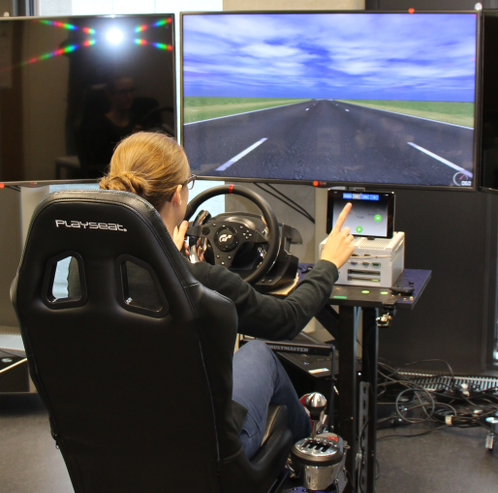
\includegraphics[width=0.7\textwidth]{images/simulator.png}
	\caption{Simulator}
	\label{fig1}
\end{figure}
%
Hierfür wurde der Demonstrator mit einem Strassenverkehrssimulator gekoppelt und somit konnten realistische Test mittels genormter Messanalysen durchgeführt werden. Aufbauend auf dem Demonstator wurden darüber hinaus zahlreiche Forschungsergebnisse im Bereich der 3D Sensordatenfusion und der mehrstufigen Klassifikation erzielt und veröffentlicht. So waren grundlegende Erkenntnisse, dass Daten aus Time-of-Flight Kameras sowohl früh als auch spät fusionieren um eine Verbesserung der Erkennungsrate zu erzielen \ref{kopinskineural}. Dieses ist insbesondere dahingehend interessant, da es unterschiedliche Performancegewinne des Systems nach sich zieht, was insbesondere für Handgestenerkennung in Echtzeit von hoher Praxisrelevanz ist. Darüber hinaus wurde mit Hilfe von mehrstufigen Neuronalen Netzen nachgewiesen, dass man Informationen aus bereits trainierten Netzen verwenden kann, um eine verbesserte Gesamtperformance des Systems zu erreichen, indem man die Erkennungsgüte mit vortrainierten Netzen stabilisiert \ref{kopinski2015pragmatic}. Diese Erkenntnisse bildeten die Grundlage für die Erkennung von Handposen und die Erkennung von dynamischen Handgesten auf Basis stabiler Posen \ref{kopinski2015real}. Letztlich wurde durch den Einsatz von Deep Learning Verfahren ein eigener Ansatz entwickelt, mittels dessen Erkenntnisse aus dem Bereich der 2D-Bilderkennung in den 3D-Raum übertragen werden konnten \ref{kopinski2016deep}.  
%
\renewcommand{\thesection}{6}
\section{Nachhaltigkeit,Übertragbarkeit}
Arbeiten zum inkrementellen Lernen
Arbeiten an Gestenerkennung
Arbeiten an Sequenzerkennung
Einfache Datensammlung
Einsetzbarkeit in der Lehre

\renewcommand{\thesection}{7}
\section{Zeitplan}

\begin{itemize}
\item Projektmanagement Maerz-Dez
\item Aufbau des Systems: Maerz - August
\item Exkursion + Workshop: September - Dezember

\end{itemize}

\renewcommand{\thesection}{8}
\section{Finanzierungsplan}
50\% Stelle Data Science E11 - TVL 11: 27.058,19
50\% Stelle Machine Learning E11 - TVL 11: 27.058,19
Sensoren 1000Euro
Rechner 15000Euro
Depermässigung
2 Hiwis 9 Monate f Visualisierung und Infrastruktur
3 1T SSD-Festplatten für Daten: 2000Euro


\renewcommand{\refname}{}
\bibliographystyle{abbrv}
\bibliography{bib}
%

\end{document}




